\subsection{Présentation d'Icube}

Icube est un laboratoire de recherche fondé en 2013 avec le soutien de l'université de Strasbourg, le CNRS, l'ENGEES et l'INSA de Strasbourg. Spécialisé dans les sciences de l'ingénieur, de l'informatique et de l'imagerie, Icube représente l'une des communauté de recherche les plus importantes avec plus de 650 membres en 2018. Les domaines de recherche du laboratoire regroupent la mécanique, la photonique, l'électronique, l'informatique, le traitement de l'image, l'automatique et la robotique, un large éventail de domaines permettant de façonner l'avenir et la société.

La recherche est organisée en 4 départements couvrant les disciplines fondamentales du laboratoire :
\begin{enumerate}
    \item{} Le département Informatique Recherche ;
    \item{} Le département Imagerie, Robotique, Télédétection et Santé ;
    \item{} Le département Électronique du Solide, Systèmes et Photonique ;
    \item{} Le département Mécanique.
\end{enumerate}

\begin{figure}[H]
    \centering
    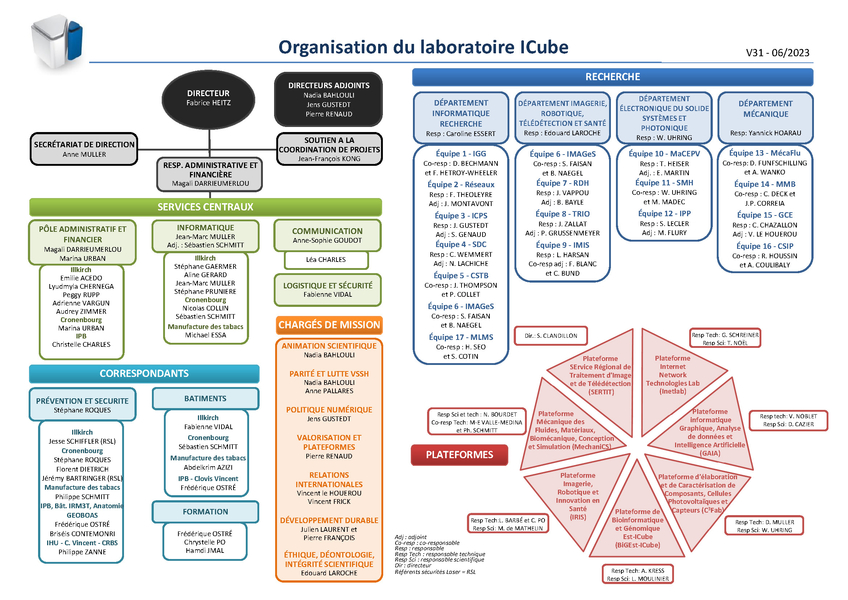
\includegraphics[scale=0.3]{figures/presentation/organigramme.jpg}
    \caption{Organigramme d'ICube}
    \label{fig1}
\end{figure}

\subsection{L'équipe reseau}

L'équipe réseau dans laquelle le stage s'est déroulé fait partie du département informatique et recherche. Cette équipe conceptualise des algorithmes et des protocoles d'architecture de communication. Ses domaines d'étude sont les réseaux de bordure, ls réseaux de cœur ainsi que les algorithmes distribués.

Cette équipe est composée de 11 membres permanents, 2 membres associés, 2 post-doctorants et 5 doctorants. Les membres permanents sont pour la plupart des enseignants-chercheurs de l'université de Strasbourg.